% ==========================================================
% Trimester 9 Term Project Report
% B.Sc. (Honours) Data Science and Artificial Intelligence
% Indian Institute of Technology Guwahati
% ==========================================================

\documentclass{article}
\usepackage{spconf,amsmath,graphicx,hyperref}

% -------------------------
% Additional useful packages
% -------------------------
\usepackage{booktabs}
\usepackage{siunitx}
\usepackage{enumitem}
\usepackage{stfloats}
\usepackage{tikz}
\usetikzlibrary{arrows.meta, positioning}

% -------------------------
% Custom definitions
% -------------------------
\def\x{{\mathbf x}}
\def\L{{\cal L}}

% -------------------------
% Title and Author Info
% -------------------------
\title{Diagnosing and Partially Mitigating Shortcut Learning in Identity
Document Fraud Detection: A Case Study from the FREUID Challenge 2026}

\name{Maheshwar Mishra (Roll Number: 23035010423)}

\address{
Term Project Report\\
Trimester 9\\[0.5em]
B.Sc. (Honours) Data Science and Artificial Intelligence\\
Indian Institute of Technology Guwahati, India\\
\texttt{m.maheshwar@op.iitg.ac.in}
}

\begin{document}
\ninept
\maketitle

% ==========================================================
% Abstract
% ==========================================================
\begin{abstract}
This report presents work carried out as a Trimester 9 term project built
around participation in the FREUID Challenge 2026 (IJCAI-ECAI), a Kaggle
competition hosted by the Microblink Fraud Lab on binary fraud detection for
identity document images. The objective was to design, train, and rigorously
evaluate a model against the competition's FREUID Score -- a metric that
specifically penalizes models which perform well globally but fail at a
strict 1\%-BPCER operating point -- and, more importantly for the academic
goals of this project, to investigate \emph{why} a model with a
near-perfect local validation score generalized poorly. The final submitted
model is a calibrated, 2-fold rank-averaged EfficientNet-B4 ensemble with
document-type and capture-modality metadata fusion, trained with a blended
focal / partial-AUC loss, reaching a public leaderboard FREUID score of
0.22090. A structured, hypothesis-by-hypothesis diagnostic investigation
(Grad-CAM, ablations, and per-image pipeline statistics) identified
shortcut learning on the face-photo region as the dominant cause of a large
gap between local validation performance and leaderboard performance, and
ruled out several plausible alternative explanations. Following the
competition's conclusion, the released private-set score (FREUID = 0.46683,
computed on 134,997 previously unseen images, roughly 17$\times$ the public
set) confirmed that this shortcut-learning weakness was not an artifact of
a small public sample, but a genuine generalization limitation. This report
documents the method, the diagnostic process, the resulting evidence, and
concrete, specific directions for future mitigation.
\end{abstract}

\begin{keywords}
Document Fraud Detection, Deep Learning, EfficientNet, Domain
Generalization, Shortcut Learning, Model Calibration, Grad-CAM
\end{keywords}

% ==========================================================
\section{Introduction}
% ==========================================================

Identity document fraud spans physical manipulations of printed documents,
GenAI-driven multimodal edits, print-and-capture ("analog hole") forgeries
that suppress digital editing artifacts by re-photographing an altered
document, and combinations of the three. Because attackers can combine
these modalities, a fraud detector that only recognizes one attack
signature -- for instance, a specific class of digital editing artifact --
will fail against the others, even if it appears highly accurate on a
validation set drawn from a similar distribution to its training data. This
makes identity document fraud detection a genuinely difficult
generalization problem, not merely a classification problem, and one with
direct practical relevance to onboarding and verification systems that rely
on automated document checks.

The FREUID Challenge 2026 (IJCAI-ECAI), organized by the Microblink Fraud
Lab~\cite{freuid2026}, poses this as binary classification -- genuine
(label 0) versus attack (label 1) -- on document images, with two metadata
fields, \texttt{is\_digital} (fully digital versus recaptured) and
\texttt{type} (country/document-type, e.g. \texttt{USA/DL}), available only
at training time. Its evaluation metric, the FREUID Score, is deliberately
constructed to penalize models that are strong overall but weak specifically
at a fixed, low false-accept operating point (Section~\ref{sec:problem}).

This project had two intertwined goals: to build a competitive submission
for the competition, and to use the project as a vehicle for demonstrating
a disciplined empirical-diagnosis process -- treating an unexplained
performance gap as a research question with falsifiable hypotheses, rather
than as a number to be improved by trial and error. Section~\ref{sec:problem}
formalizes the task and metric. Section~\ref{sec:method} details the model,
training pipeline, and inference procedure. Section~\ref{sec:experiments}
reports quantitative results, including the post-competition private-set
score. Section~\ref{sec:discussion} presents the diagnostic investigation
that forms the core empirical contribution of this report. Section~\ref{sec:conclusion}
concludes and outlines specific, evidence-motivated future work.

% ==========================================================
\section{Problem Statement and Objectives}
\label{sec:problem}
% ==========================================================

\subsection{Problem Statement}

Given an identity document image, and metadata fields \texttt{is\_digital}
and \texttt{type} available at training time only, predict a continuous
fraud score in $[0,1]$ (higher indicates more likely fraudulent). The
private test set is known in advance to contain two document types absent
from both the training data and the public test set, so any solution must
generalize to genuinely unseen document formats, not merely to unseen
individual images of known formats.

Performance is measured by the \textbf{FREUID Score} (lower is better),
defined as one minus the harmonic mean of two complementary error terms:
\begin{align}
g_{\text{audet}} &= 1 - \text{AuDET} \\
g_{\text{apcer}} &= 1 - \text{APCER@1\%BPCER} \\
\text{FREUID} &= 1 - \frac{2 \cdot g_{\text{audet}} \cdot g_{\text{apcer}}}{g_{\text{audet}} + g_{\text{apcer}}}
\end{align}
where AuDET is the area under the Detection Error Trade-off curve (an
overall ranking-quality measure, analogous to $1{-}$AUC-ROC in spirit) and
APCER@1\%BPCER is the attack-miss rate at the fixed operating point where
the genuine-sample false-accept rate (BPCER) is 1\%. Because FREUID is a
harmonic mean of the two error terms, a model that is strong globally
(low $g_{\text{audet}}$) but weak specifically at the 1\%-BPCER operating
point (high $g_{\text{apcer}}$) is penalized heavily -- global ranking
quality alone is an insufficient training objective for this metric, which
directly shaped the loss design in Section~\ref{sec:loss} and the decision
to treat post-hoc calibration as mandatory rather than optional
(Section~\ref{sec:calibration}).

\subsection{Objectives}
\begin{enumerate}[noitemsep]
    \item Design and train a document-fraud classifier that fuses visual
    features with document-type and capture-modality metadata, robust to
    both digital and print-and-capture attack modalities.
    \item Implement a training and calibration pipeline that directly
    targets the FREUID metric's low-false-accept operating point, rather
    than optimizing a loosely correlated proxy such as plain accuracy or
    global AUC.
    \item Build a local evaluation harness that exactly reproduces the
    competition's scoring logic, broken down by document type and capture
    modality, to enable meaningful ablations.
    \item Diagnose, with falsifiable, isolated experiments, the cause of any
    gap between local validation performance and leaderboard performance,
    rather than treating such a gap as an accepted but unexplained cost of
    doing the competition.
    \item Produce a reproducible artifact (open-source code, frozen
    checkpoints, Docker-based inference package) satisfying the
    competition's prize-eligibility requirements.
\end{enumerate}

% ==========================================================
\section{Methodology}
\label{sec:method}
% ==========================================================

\subsection{Data}

All training data is the competition-provided FREUID dataset; no external
or proprietary datasets were used. \texttt{train\_labels.csv} provides
\texttt{id}, \texttt{image\_path}, \texttt{label}, \texttt{is\_digital}, and
\texttt{type}. The majority of observed document types share a
driver's-license-style layout; one type, \texttt{MAURITIUS/ID}, is the only
ID-card-format type in the dataset -- a structural difference that becomes
relevant to a diagnostic finding in Section~\ref{sec:pipeline-fingerprint}.
Folds for cross-validation are constructed via stratified $k$-fold sampling
on a composite key of \texttt{label} $\times$ \texttt{is\_digital}
$\times$ \texttt{type}, so that every fold observes every combination of
attack type, capture modality, and document format present in training.

\subsection{Architecture}

\begin{figure}[t]
\centering
\resizebox{\linewidth}{!}{%
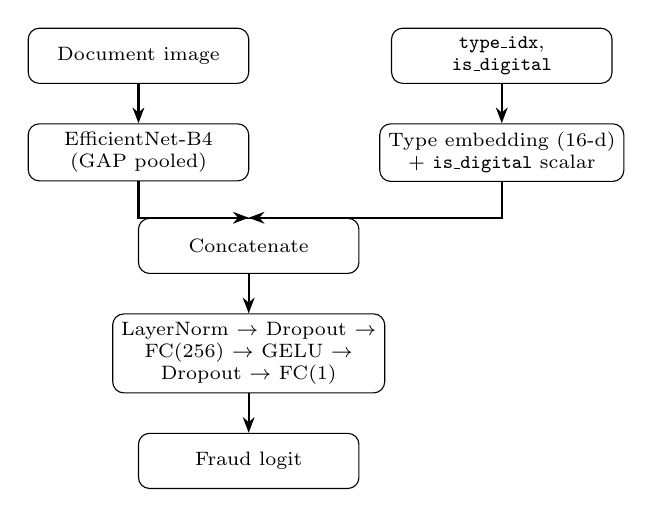
\begin{tikzpicture}[
    box/.style={draw, rounded corners, minimum height=0.7cm, minimum width=2.8cm, align=center, font=\scriptsize, inner sep=3pt},
    arrow/.style={-{Stealth[length=2mm]}, thick}
]
\node[box] (img) {Document image};
\node[box, below=0.5cm of img] (backbone) {EfficientNet-B4\\(GAP pooled)};

\node[box, right=1.8cm of img] (meta) {\texttt{type\_idx},\\\texttt{is\_digital}};
\node[box, below=0.5cm of meta] (embed) {Type embedding (16-d)\\+ \texttt{is\_digital} scalar};

\node[box, below=1.7cm of img, xshift=1.4cm] (concat) {Concatenate};
\node[box, below=0.5cm of concat] (head) {LayerNorm $\to$ Dropout $\to$\\FC(256) $\to$ GELU $\to$\\Dropout $\to$ FC(1)};
\node[box, below=0.5cm of head] (out) {Fraud logit};

\draw[arrow] (img) -- (backbone);
\draw[arrow] (meta) -- (embed);
\draw[arrow] (backbone.south) |- (concat.north);
\draw[arrow] (embed.south) |- (concat.north);
\draw[arrow] (concat) -- (head);
\draw[arrow] (head) -- (out);
\end{tikzpicture}%
}
\caption{Model architecture: EfficientNet-B4 visual features fused with
document-type embedding and capture-modality scalar via a small MLP head.}
\label{fig:architecture}
\end{figure}

The backbone is \texttt{tf\_efficientnet\_b4}~\cite{tan2019efficientnet}
(via \texttt{timm}, Apache-2.0 licensed), ImageNet-pretrained, with the
classifier head removed and global average pooling retained. A
document-type embedding (16-dimensional, with index 0 reserved as a padding
/ "unknown" slot for document types unseen at training time) and the
\texttt{is\_digital} scalar are concatenated with the pooled backbone
features, followed by LayerNorm $\to$ Dropout $\to$ Linear(256) $\to$ GELU
$\to$ Dropout $\to$ Linear(1), producing a single fraud logit
(Figure~\ref{fig:architecture}).

\subsection{Input and Augmentation}

Images are resized to $320 \times 320$. Training augmentation combines
standard spatial transforms (horizontal flip, shift/scale/rotate, coarse
dropout) with a physics-inspired "recapture" pipeline -- motion/Gaussian/
defocus blur, sensor noise, JPEG recompression, perspective warp, and
moir\'e-pattern simulation -- intended to teach the model that these
capture-pipeline degradations alone are not evidence of fraud, rather than
allowing it to key on recapture artifacts as a shortcut. A face-region
occlusion augmentation, added specifically in response to the diagnostic
finding in Section~\ref{sec:shortcut} (face bounding boxes precomputed once
via Haar cascade, then randomly masked or Gaussian-blurred with probability
0.3 during training only), was intended to reduce reliance on the
face-photo region.

\subsection{Loss}
\label{sec:loss}

A blended loss, $(1-w)\cdot\text{FocalLoss} + w\cdot\text{PartialAUCLoss}$
with $w=0.5$, is used. Focal loss ($\alpha{=}0.75$, $\gamma{=}2.0$)
addresses class imbalance and down-weights easy negatives~\cite{lin2017focal}.
The partial-AUC term is a margin-based pairwise ranking loss restricted to
the hardest genuine samples -- the top 10\% by predicted score, i.e. the
samples most likely to set the 1\%-BPCER threshold -- adapted from the
large-scale partial-AUC surrogate formulation of Yao et
al.~\cite{yao2022pauc}, chosen specifically because it targets the same
low-false-accept region the FREUID metric penalizes, rather than optimizing
a metric such as plain cross-entropy or global AUC that is only loosely
correlated with it.

\subsection{Calibration}
\label{sec:calibration}

APCER@1\%BPCER depends on the score distribution near a specific decision
threshold, not merely on ranking quality -- a perfectly-ranked but
poorly-scaled model can still fail this operating point. Post-hoc
calibration is therefore treated as mandatory: temperature
scaling~\cite{guo2017calibration} is fit per fold on that fold's own
held-out validation logits (never on training data), minimizing negative
log-likelihood via L-BFGS-B.

\subsection{Inference and Ensembling}

Test-time metadata is unknown by construction: \texttt{is\_digital} and
\texttt{type} are set to the padding/"unknown" slot for every test image,
including the two document types confirmed present in the private test set
but absent from train and public test. An ablation found this has
negligible effect on FREUID score (Section~\ref{sec:ruled-out}). Test-time
augmentation averages logits over the original image and a horizontal flip
prior to calibration. The submitted model is a 2-fold ensemble: each fold
is trained, validated, and calibrated independently, and final scores are
the \emph{rank average} (not a raw probability average) of the two folds'
calibrated, TTA-averaged scores, chosen for robustness to any residual
inter-fold calibration-scale mismatch.

% ==========================================================
\section{Experiments and Results}
\label{sec:experiments}
% ==========================================================

\subsection{Experimental Setup}

Training was run on Kaggle notebooks (single T4 GPU), with mixed-precision
training, gradient accumulation (effective batch size 32), and a linear-warmup/
cosine-annealing learning-rate schedule. Early stopping (patience 4 epochs,
minimum FREUID improvement 0.001) was used once diagnostic runs showed both
folds plateauing by epoch 7--9. All reported local metrics are computed with
a from-scratch, locally-implemented FREUID Score function, validated on
synthetic random and near-perfect score distributions before use, so that
every validation fold is scored exactly as the competition scores
submissions.

\subsection{Results}

\begin{table}[t]
\centering
\caption{Per-fold local validation metrics for the submitted model, at
export time.}
\label{tab:fold-metrics}
\begin{tabular}{@{}lccc@{}}
\toprule
Fold & Best epoch & Local val. FREUID & Temperature \\
\midrule
0 & 17 & 0.000274 & 1.0 \\
1 & 8  & 0.000683 & 1.0 \\
\bottomrule
\end{tabular}
\end{table}

\begin{table}[t]
\centering
\caption{Leaderboard results. Public and private scores are computed by
Kaggle against held-out ground truth not available locally.}
\label{tab:lb-results}
\resizebox{\linewidth}{!}{%
\begin{tabular}{@{}lcc@{}}
\toprule
Submission & Public LB FREUID $\downarrow$ & Private LB FREUID $\downarrow$ \\
\midrule
Prize-eligible final (\texttt{v4.csv}) & 0.22090 & --$^{\text{a}}$ \\
Full-set inference (\texttt{v4\_FINAL.csv}) & 0.21868 & 0.46683 \\
\bottomrule
\end{tabular}%
}
\end{table}
\vspace{-0.3cm}
\noindent{\scriptsize $^{\text{a}}$Private score for this exact submission is not
separately available; the full-set inference run below is the directly
comparable measurement, differing from the prize-eligible submission only
in that all 134,997 private-portion rows received real model predictions
rather than a constant placeholder value.}

Table~\ref{tab:fold-metrics} shows both folds converging to near-ceiling
local validation FREUID scores. Table~\ref{tab:lb-results} shows the public
leaderboard score (0.21868--0.22090 across the two closely related
submissions) and, following the competition's conclusion, the private
leaderboard score of 0.46683 -- computed on 134,997 images, roughly
$17\times$ the size of the 7,821-image public set, and including two
document types never seen during training. The gap between local validation
(order $10^{-4}$) and even the public leaderboard score (order $10^{-1}$)
was already large enough during development to warrant investigation; the
subsequent private-score result is discussed in relation to that
investigation in Section~\ref{sec:gap-confirmed}.

% ==========================================================
\section{Discussion: Diagnosing the Local-Validation-to-Leaderboard Gap}
\label{sec:discussion}
% ==========================================================

Rather than accepting the local-validation-to-leaderboard gap as an
unexplained fact of the competition, a structured sequence of isolated,
falsifiable diagnostics was run, each targeting one specific hypothesis.
Table~\ref{tab:versioning} summarizes the resulting notebook-versioning
trail; diagnostic sub-steps within each version are described inline where
relevant below rather than enumerated separately.

\begin{table}[t]
\centering
\caption{Notebook-versioning trail for the diagnostic investigation.}
\label{tab:versioning}
\resizebox{\linewidth}{!}{%
\begin{tabular}{@{}ll@{}}
\toprule
Version & Purpose \\
\midrule
v1 $\to$ v2 & Initial training pipeline; v2 moved to full-resolution \\
            & ($320^2$) production training. \\
v3 & Diagnostics: leakage checks, train/val duplicate-image \\
   & checks, global pipeline-fingerprint checks, Grad-CAM. \\
v4 & \textbf{Frozen/submitted model} --- adds face-region \\
   & occlusion augmentation and early stopping on top of v2. \\
v5 & Diagnostic: \texttt{is\_digital} test-time flag ablation. \\
v6 & Diagnostic: Grad-CAM re-check of learned attention. \\
v7 & Diagnostic: per-document-type pipeline/noise statistics. \\
v8 & Mitigation attempt: noise/sharpness-equalizing fine-tune \\
   & warm-started from v4 --- inconclusive, not adopted. \\
\bottomrule
\end{tabular}%
}
\end{table}

\subsection{Root Cause: Face-Region Shortcut Learning}
\label{sec:shortcut}

Grad-CAM~\cite{selvaraju2017gradcam} applied to the trained model shows
consistent, tightly localized attention on the face-photo region for
fraud-labeled examples, and diffuse attention toward background and border
regions for genuine examples. This is consistent with the model having
learned a narrow face-region anomaly detector rather than a general
document-fraud detector: near-perfect local validation reflects strong
separability on this one detectable manipulation signature, which does not
fully generalize to the broader distribution of attack types (physical
manipulation, GenAI multimodal edits, print-and-capture) present in the
hidden test set. Face-region occlusion augmentation was added in response
to this finding (Section~\ref{sec:method}), but, as discussed in
Section~\ref{sec:gap-confirmed}, only partially mitigated the effect.

\subsection{Ruled-Out Hypotheses}
\label{sec:ruled-out}

Several other plausible explanations for the gap were tested and rejected
before converging on Section~\ref{sec:shortcut}:
\begin{itemize}[noitemsep]
    \item \textbf{Metadata leakage.} Zeroing \texttt{is\_digital} and/or
    \texttt{type\_idx} at inference time produced only a noise-level change
    in leaderboard score (v5, \texttt{is\_digital} test-time flag ablation:
    public LB FREUID 0.21941 versus the frozen v4 model's 0.22090, a delta
    of 0.00149), ruling out reliance on these fields as a shortcut.
    \item \textbf{Train/validation image duplication.} Perceptual-hash
    matches between splits were investigated and found to be false
    positives from shared document templates (identical layout, different
    content), not literal duplicate images.
    \item \textbf{Global pipeline fingerprints.} File size, resolution,
    JPEG quality, and FFT high-frequency energy were compared between
    fraud and genuine classes and found essentially identical, ruling out
    a trivial global compression or capture fingerprint.
    \item \textbf{Submission pipeline bug.} After the competition
    concluded, the large public/private gap was initially suspected to be
    caused by an inference-pipeline error (private-portion rows retaining a
    placeholder fill value). Submission logs were checked directly and
    confirmed \texttt{real=142818} predicted rows and zero placeholder
    fallbacks, ruling this out as an explanation.
\end{itemize}

\subsection{Secondary Finding: A Document-Type Pipeline Fingerprint}
\label{sec:pipeline-fingerprint}

A further diagnostic found that \texttt{MAURITIUS/ID} -- the only
ID-card-format type in the dataset -- is statistically distinct from all
other types in noise standard deviation, Laplacian-variance sharpness, FFT
high-frequency energy ratio, and intensity statistics, independent of
label. JPEG quality, by contrast, was identical across types, ruling out a
simple compression-setting explanation. This is most consistent with a
rendering- or capture-pipeline difference specific to that document format
rather than a fraud-specific cue, but was not corrected before the
competition's code-freeze deadline and is reported as a known, open
limitation (Section~\ref{sec:future-work}).

\subsection{The Private-Set Result Confirms the Diagnosis}
\label{sec:gap-confirmed}

The private leaderboard score released after the competition's conclusion
(FREUID = 0.46683, Table~\ref{tab:lb-results}) is consistent with, and
substantially strengthens, the shortcut-learning diagnosis of
Section~\ref{sec:shortcut}, for three compounding reasons. First, scale:
the private set is roughly $17\times$ larger than the public set, so a
small public sample landing favorably by chance is far less likely to
recur at scale, and the larger sample should more closely reflect the
model's true generalization behavior. Second, the private set is confirmed
to contain two document types entirely absent from training, which by
design are routed through the model's "unknown"-type embedding slot --
a genuine generalization stress test the model had not encountered at all
during training. Third, the face-occlusion mitigation added in response to
Section~\ref{sec:shortcut} was explicitly partial by design ($p{=}0.3$,
i.e. roughly 70\% of training images still show an unoccluded face region),
so residual reliance on the shortcut was expected, not merely possible.
Taken together, the roughly three-orders-of-magnitude gap between local
validation FREUID and public leaderboard FREUID, and the further
degradation to the private leaderboard score, is attributable primarily to
incompletely mitigated shortcut learning rather than to a conventional
train/test distribution shift, a calibration failure, or a submission
pipeline defect -- each of the latter was directly tested and ruled out or
shown to be a comparatively minor effect.

% ==========================================================
\section{Conclusion and Future Work}
\label{sec:conclusion}
% ==========================================================

This project produced a competitive FREUID Challenge submission (public
leaderboard FREUID 0.21868--0.22090) and, more centrally to its academic
goals, a disciplined, hypothesis-by-hypothesis diagnostic process that
converted an initially opaque local-validation-to-leaderboard gap into a
specific, evidenced explanation: shortcut learning on the face-photo
region, confirmed and amplified at the much larger private-test-set scale,
compounded by a secondary, unresolved document-type pipeline fingerprint.
Several plausible alternative explanations -- metadata leakage, data
duplication, global pipeline artifacts, and a submission-pipeline defect --
were each explicitly tested and ruled out rather than assumed. The
project's main learning outcome was methodological: that a large,
initially unexplained gap between a locally-measured metric and a
held-out evaluation is itself a research question, answerable with the
same isolated-hypothesis discipline used elsewhere in the pipeline, rather
than something to be patched over with more training epochs or more
data augmentation applied indiscriminately.

\subsection{Future Work}
\label{sec:future-work}

Two concrete, specific extensions follow directly from the diagnostic
findings above and are proposed here as future work, distinct from work
completed within this report:
\begin{enumerate}[noitemsep]
    \item \textbf{Direct face-shortcut mitigation.} An auxiliary loss term
    that explicitly penalizes face-region-only predictive power (e.g. by
    training a small auxiliary head on face-region crops alone and
    penalizing its accuracy), or a dedicated ensemble member trained with
    the face region always masked rather than masked with probability 0.3,
    would more directly target the root cause identified in
    Section~\ref{sec:shortcut} than the partial occlusion augmentation used
    here.
    \item \textbf{Targeted pipeline-fingerprint correction.} Rather than a
    uniform, untargeted augmentation, a per-image adaptive correction --
    scaling noise/sharpness/intensity adjustments to each image's measured
    deviation (via robust median/median-absolute-deviation statistics) from
    the global distribution on the four axes identified in
    Section~\ref{sec:pipeline-fingerprint} -- would concentrate the
    intervention specifically on outlier document types such as
    \texttt{MAURITIUS/ID}, rather than perturbing the entire dataset
    uniformly. A fully symmetric warm-start fine-tune, in which every fold
    is fine-tuned from an identical, frozen starting checkpoint with an
    identical epoch budget, would additionally be needed to obtain a clean,
    directly comparable before/after measurement.
\end{enumerate}
An initial attempt at combining both directions above was made following
the competition's conclusion but did not complete successfully within the
available compute session before this report was finalized; it is
reported here as a well-motivated future direction rather than as a
completed experiment with results.

% ==========================================================
\section{Artifacts and Demonstrations}
% ==========================================================

\begin{itemize}[noitemsep]
    \item \textbf{Code Repository:} \url{https://github.com/MaheshwarMahi/freuid-fraud-detection}
    \item \textbf{Reproducibility Repository:} \url{https://github.com/MaheshwarMahi/freuid-challenge-2026-reproducibility}
    \item \textbf{Competition Page:} \url{https://kaggle.com/competitions/the-freuid-challenge-2026-ijcai-ecai}
\end{itemize}

\textbf{Note:} AI-assisted tools were used during this project for code
scaffolding, debugging assistance, and drafting support. All modeling
decisions, diagnostic hypotheses, and interpretations of results are the
author's own.

% ==========================================================
% References
% ==========================================================
\vfill\pagebreak
{\fontsize{8}{9}\selectfont
\bibliographystyle{IEEEbib}
\bibliography{refs}
}

\end{document}
